% ERA-Großpraktikums: Benutzeranleitung -- Features

\section{Features}

\subsection*{Überblick}
\todo[inline]{Am besten mit Bild und nummerierten Pfeilen}

% Ich schlage eine Teilung der einzelnen Features nach Projektverwaltung(Laden, Speichern, Snapshots), Erstellen von Programmen (Editor, Hilfetexte), Ausführung von Programmen(Ausfühmodi, Breakpoints), Interaktion mit laufenden Programmen (Input/Output-Components) und sonstiges vor

\subsection{Projekt}

\subsubsection{Projekt erstellen}
\todo[inline]{V.a. Projekt erstellen: Auswahl Architektur, Bitlänge, Modlue, Parser, etc.}

\subsubsection{Speichern/Laden}
\todo[inline]{Speichern/Laden von Projekt und Code}

\subsubsection{Snapshots}
\todo[inline]{Speichern/Laden + Was ist das?; Welche Eigenschaften muss mein erstelltes Projekt haben, damit ich SnapshotXY laden kann (passende Architektur/passende Module)}


\subsection{Erstellen von Programmen}

\subsubsection{Editor}
\todo[inline]{Alles zum Editor (zoomen, Makros aufklappen, Fehlermeldungen anzeigen, Tooltips etc)}

\subsubsection{Hilfetextkomponente}
\todo[inline]{Was wird angezeigt, zu welchem Befehl (Zeile!), wann (nach dem Parsen)}


\subsection{Ausführung von Programmen}

\subsubsection{Ausführungsmodi}
\todo[inline]{komplett, schritt-für-schritt, zum nächsten breakpoint; hier am besten mmit bildern der einzelnen Knöpfe}

\subsubsection{Registerkomponente}
\todo[inline]{Alles zu den Registerkomponenten, wie verstelle ich die Zahlendarstellung, Highlight bei Änderung etc}

\subsubsection{Speicherkomponente}
\todo[inline]{Alles zur Speicherkomponente: Wie verstelle ich die Zahlendarstellung, Hinzufügen/Entfernen von Spalten}


\subsection{Interaktion mit laufenden Programmen}
\todo[inline]{Hier sollte (für alle Komponenten ja gleich) die Einstellungsmöglichkeiten (Zahnrad-knopf) und welches Symbol welche Komponente bedeutet}

\subsubsection{Eingabe -- Pfeiltasten}
\todo[inline]{v.a. welche Werte werden für welchen Pfeil geschrieben}

\subsubsection{Eingabe -- Mausklick}
\todo[inline]{welche werte werden geschrieben, Reihenfolge?}

\subsubsection{Eingabe -- Text}
\todo[inline]{wann wird geschriebener Text in den Speicher geschrieben?, Wie lang kann mein Text sein?}

\subsubsection{Ausgabe -- Lichtbandanzeige}
\todo[inline]{besondere Einstellungen! Farbwahl! Manuelles setzen der Strips möglich!}

\subsubsection{Ausgabe -- 7-Segmentanzeige}
Die sogenannte 7-Segment Anzeige ist eine einfache alphanumerische Ausgabe, 
wie sie häufig bei kleinen digitalen Geräten zum Einsatz kommt.
Anzeige besteht, wie der Name schon sagt, aus 7 Strichen, die unabhängig voneinander zum Leuchten gebracht werden können.

\begin{figure}[ht]
	\centering
  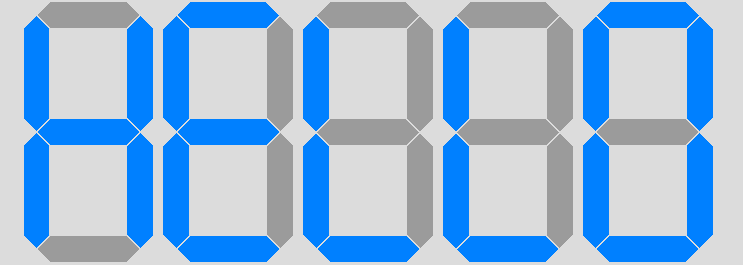
\includegraphics[width=0.8\textwidth]{Images/7-Segment_Hello}
	\caption{Die 7-Segment Anzeige im Simulator}
	\label{7-Segment}
\end{figure}

Jedes dieser Segmente wird durch ein einzelnes Bit angesteuert. Dabei bedeutet $1$, dass das Segment leuchten soll und $0$ entsprechend, dass es nicht leuchten soll.
Pro Zeichen wird somit 8 Byte zum Ansteuern benötigt, wobei das höchstwertige Bit in der Regel ignoriert wird.

Wenn man die Maus im Simulator über ein Zeichen bewegt, erscheint dort die Reihenfolge, in der die Bits den einzelnen Segmenten zugeordnet sind.

\begin{figure}[ht]
	\centering
  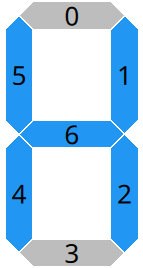
\includegraphics[width=0.2\textwidth]{Images/7-Segment_Hover}
	\caption{Die Reihenfolge der Bits}
	\label{7-Segment_Hover}
\end{figure}

Es können auch gleichzeitig mehrere Zeichen angesteuert werden. Die einzelnen Bytes für jedes Zeichen stehen dann im Speicher an aufeinanderfolgenden Adressen.
Dabei muss aber darauf geachtet werden, dass die Reihenfolge genau umgedreht ist. Das Zeichen am rechten Rand steht somit an der ersten Adresse im Speicher, 
danach folgt das vorletzte usw.

\begin{warningblock}{Reihenfolge der Zeichen}
Die Ansteuerung der Zeichen ist genau geschieht (wie im Zahlensystem) von rechts nach links. 
\end{warningblock}

Ein kleines Beispiel verdeutlicht dies wohl am besten.

\begin{exampleblock}{HELLO}
	Für das oben gezeigte \texttt{HELLO} wäre also folgende Ansteuerung nötig:\\
	\begin{tabular}{llll}
	0x3f & 0b00111111 & & \texttt{O}\\
	0x38 & 0b00111000 & & \texttt{L}\\
	0x38 & 0b00111000 & & \texttt{L}\\
	0x79 & 0b01111001 & & \texttt{E}\\
	0x76 & 0b01110110 & & \texttt{H}\\
	\end{tabular}
\end{exampleblock}

Falls man sich den Umweg über die Ansteuerung über Speicheradressen sparen möchte, 
kann man die einzelnen Leuchtsegmente auch durch einen Klick mit der linken Maustaste aktivieren bzw. deaktivieren. 

Für die Anzeige gibt es zwei Einstellungen, die man über das Zahnrad rechts unten aufrufen kann:\\
\begin{itemize}
\item \texttt{Memory Source (Address):} definiert den Speicherbereich, der für die 7-Segment Ausgabe herangezogen wird. Default ist 0.
\item \texttt{Number of Digits:} die Anzahl der angezeigten 7-Segment Zeichen. Für jedes der Zeichen wird ein Byte im Speicher benötigt. 
					Die Bytes für jedes Zeichen sind im Speicher an aufeinanderfolgenden Adressen ab der gewählten  \texttt{Memory Source Address} angeordnet.
\end{itemize}



\subsubsection{Ausgabe -- Konsole}
\todo[inline]{pipe-like, array-based; }


\subsection{Sonstige Features}